\section{Networking}

Here are various network architectures:
\begin{enumerate}
    \item \textit{Monolithic app}: this setup requires minimal network resources and relies on proprietary protocols.
    \item \textit{Client-server}: high network demands within the enterprise, applications confined within the enterprise, and a combination of TCP/IP and proprietary protocols.
    \item \textit{Web applications}: utilizes ubiquitous TCP/IP, accessible from anywhere, and servers are segmented into multiple units.
    \item \textit{Microservices}: infrastructure shifts to cloud providers, servers segmented into microservices, resulting in increased server-to-server traffic.
\end{enumerate}
A data center comprises all physical infrastructure necessary to support cloud computing services. 
This infrastructure is typically co-located within a room, building, or set of adjacent buildings.
Applications within the data center may include: cloud computing, cloud storage, and web services. 
These applications facilitate the consolidation of computation and network resources, often in very large data centers ranging from 1,000 to 1,000,000 servers.

\paragraph*{Demand increasing}
As server performance improves over time, there is a natural increase in demand for inter-server bandwidth. 
By doubling the number of compute or storage elements, we can easily double the aggregate compute capacity or storage.

However, networking poses a challenge for straightforward horizontal scaling. 
While doubling leaf bandwidth is straightforward—by doubling the number of servers, we also double the network ports and thus the bandwidth—dealing with bisection bandwidth becomes more complex when assuming that every server needs to communicate with every other server.
\begin{definition}[\textit{Bisection bandwidth}]
    Bisection bandwidth refers to the bandwidth across the narrowest line that evenly divides the cluster into two parts. 
\end{definition}
This metric serves as a characterization of network capacity, as it represents the capacity for randomly communicating processors to transmit data across the central portion of the network. 
When assuming that every server must communicate with every other server, it becomes necessary to double not only leaf bandwidth but also bisection bandwidth.

\paragraph*{Datacenter networking}
Data center networking can be categorized into three primary types:
\begin{itemize}
    \item \textit{Switch-centric architectures}: utilize switches for packet forwarding tasks.
    \item \textit{Server-centric architectures}: employ servers equipped with multiple Network Interface Cards (NICs) to serve as switches alongside their computational functions.
    \item \textit{Hybrid architectures}: blend both switches and servers to handle packet forwarding duties.
\end{itemize}

\subsection{Switch-centric architecture}
\begin{figure}[H]
    \centering
    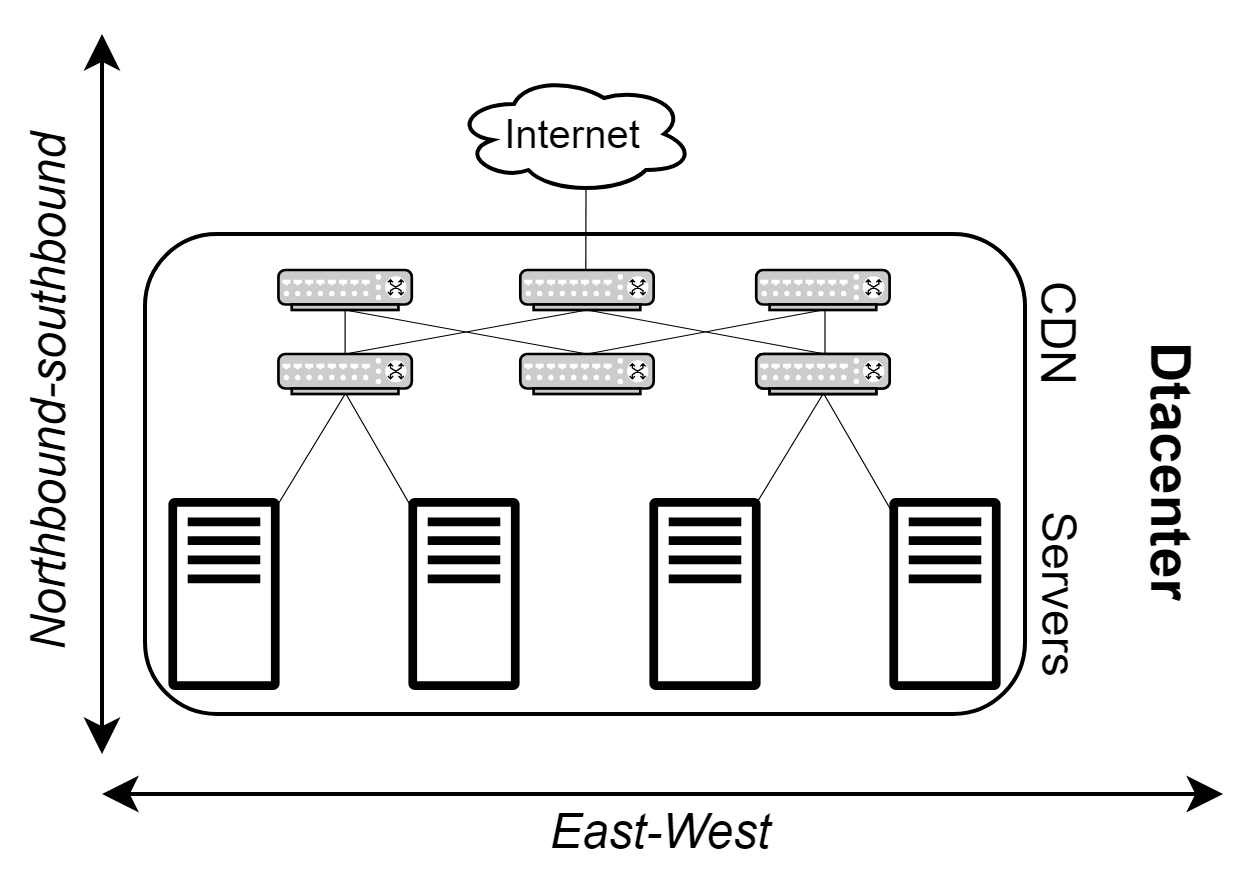
\includegraphics[width=0.6\linewidth]{images/sc.png}
    \caption{Switch-centric architecture}
\end{figure}
The traffic is divided into two main flows: 
\begin{itemize}
    \item Northbound-southbound: direct connection between internet and servers. 
    \item East-West: inter-server communication within a data center, often referred to as East-West traffic, involves several key aspects:
        \begin{itemize}
            \item Storage replication, typically characterized by numerous data flows with relatively few instances of data.
            \item In distributed file systems like Hadoop, maintaining at least three copies of the same data, commonly with two copies residing within the same rack and one in a different rack.
            \item Virtual Machine (VM) migration, a process integral to tasks such as Network Function Virtualization (NFV), where data undergoes processing across a series of VMs, such as firewalls, web servers, parental control systems, and accounting servers.
        \end{itemize}
        It's notable that East-West traffic typically surpasses North-South traffic in terms of volume and significance within the data center environment.
        This type of traffic can be: unicast, multicast, and incast. 
\end{itemize}

\subsection{Classical 3-tier architecture}
The classical 3-tier switch-centric architecture is structured into three distinct layers, as illustrated in the diagram below:
\begin{figure}[H]
    \centering
    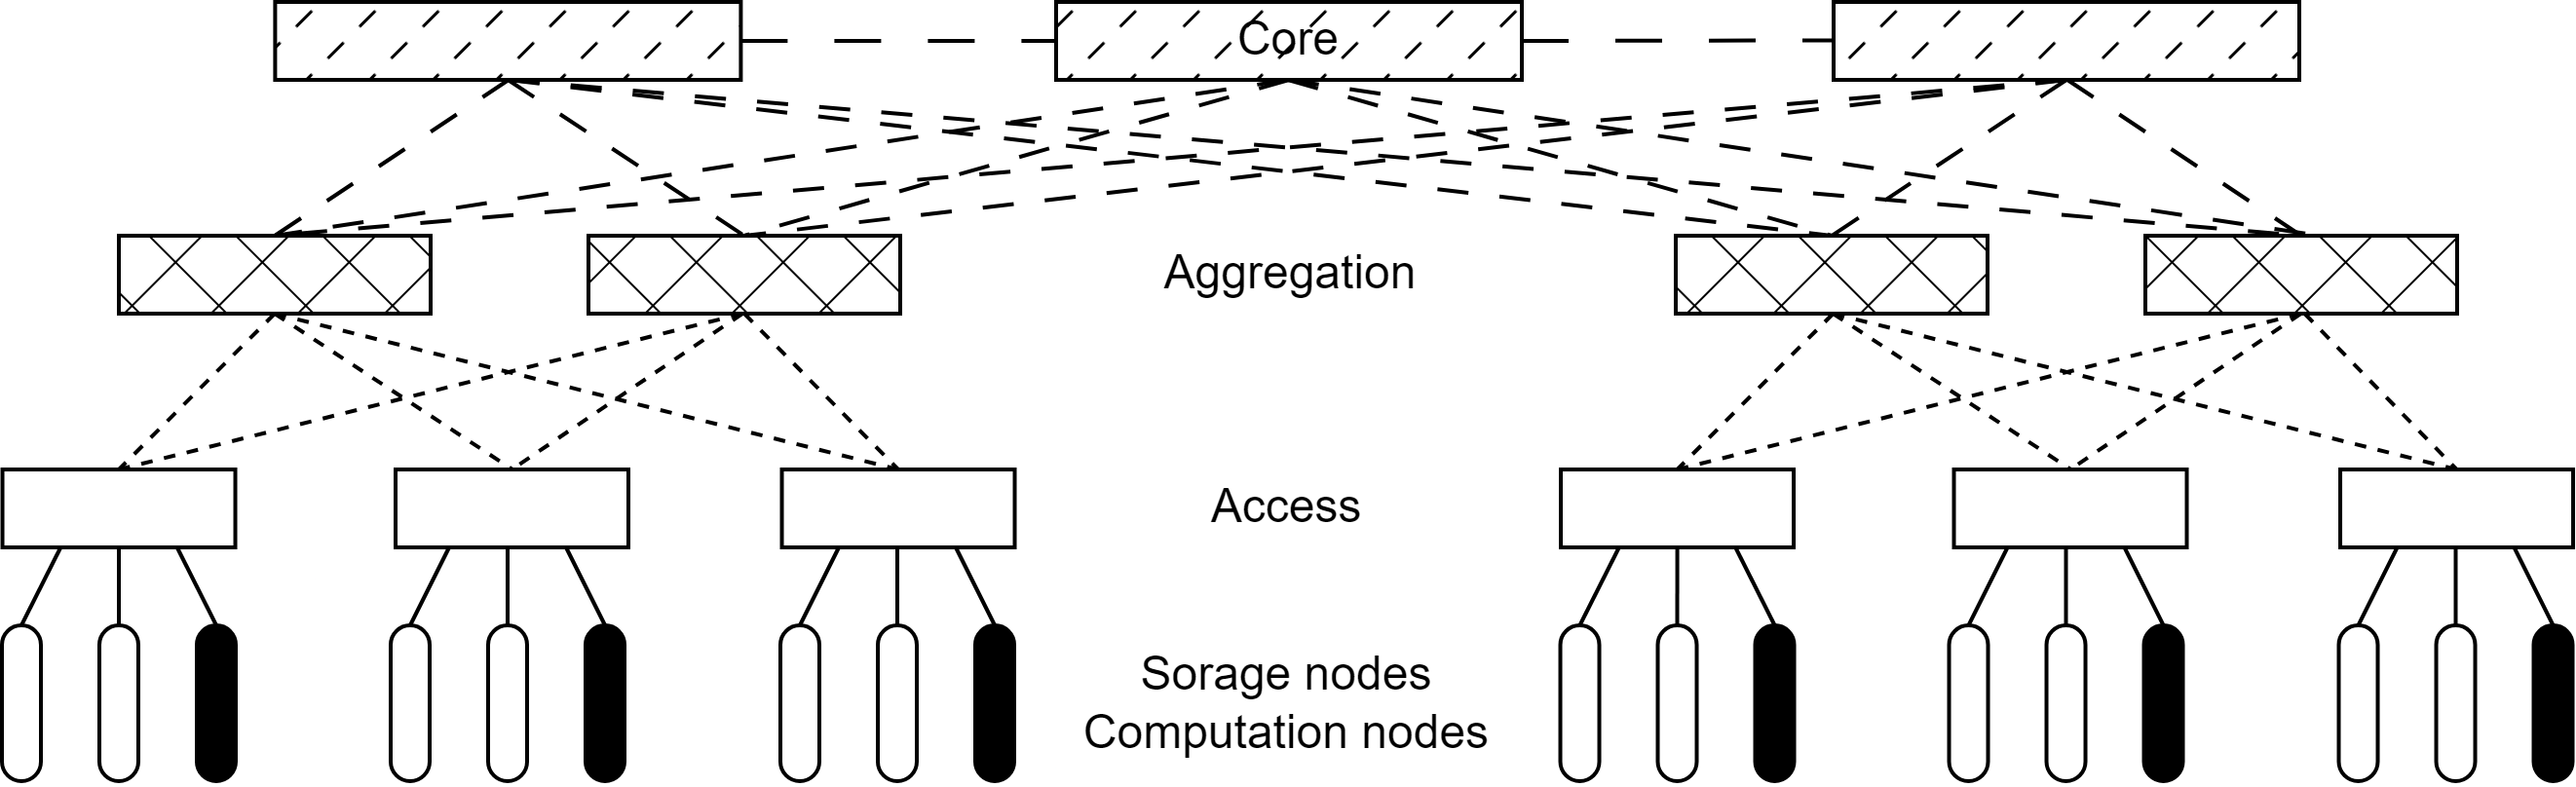
\includegraphics[width=0.75\linewidth]{images/sca.png}
    \caption{Classical 3-tier architecture} 
\end{figure}
This configuration represents a straightforward Data Center Network (DCN) topology, where servers interface with the DCN via access switches.
Each access-level switch links to a minimum of two aggregation-level switches, which, in turn, connect to core-level switches (gateways).

\paragraph*{Server structure}
Servers can be categorized into two main architectures:
\begin{itemize}
    \item \textit{Top-of-Rack} (ToR): in a rack, all servers are linked to a Top-of-Rack (ToR) access switch, with both the servers and the ToR switch situated within the same rack.
        Aggregation switches are housed either in dedicated racks or in shared racks alongside other ToR switches and servers. 
        This setup restricts the number of cables, resulting in simpler cabling. 
        Moreover, the number of ports per switch is constrained, leading to lower costs. 
        However, this configuration suffers from limited scalability and heightened complexity in switch management due to the proliferation of switches.
    \item \textit{End-of-Row} (EoR): aggregation switches are strategically placed at the end of each corridor, serving as the termination point for a row of racks. 
        Servers within racks establish direct connections to the aggregation switch situated in another rack. 
        Due to this arrangement, aggregation switches require a greater number of ports, resulting in more intricate cabling and necessitating longer cables, which in turn incur higher costs. 
        Typically, a patch panel is employed to facilitate connections between servers and the aggregation switch. 
        Despite the more complex cabling, this setup offers simpler switch management owing to the reduced number of switches involved.
\end{itemize}

\paragraph*{Bandwidth increasing}
Boosting bandwidth can be achieved through various methods. 
Firstly, augmenting the number of switches at both the core and aggregation layers facilitates enhanced bandwidth. 
Additionally, employing routing protocols like Equal Cost Multiple Path (ECMP) enables equitable distribution of traffic across various routes, further amplifying bandwidth capabilities.
While this solution is straightforward, it can prove to be exceedingly costly in expansive data centers for several reasons:
\begin{itemize}
    \item The upper layers necessitate swifter network equipment, which tends to be more expensive.
    \item Each layer is serviced by switches of varying types, compounding acquisition costs and introducing complexities in management, spare-part stocking, and energy consumption.
\end{itemize}
Cumulatively, these factors contribute to significantly elevated expenses, both in terms of upfront investments and ongoing operational costs.

\subsection{Leaf-spine architecture}
The Leaf-spine switch-centric architecture is structured into two distinct layers: 
\begin{itemize}
    \item Leaf: ToR switch
    \item Spine: dedicated switches (aggregation switches)
\end{itemize}
\begin{figure}[H]
    \centering
    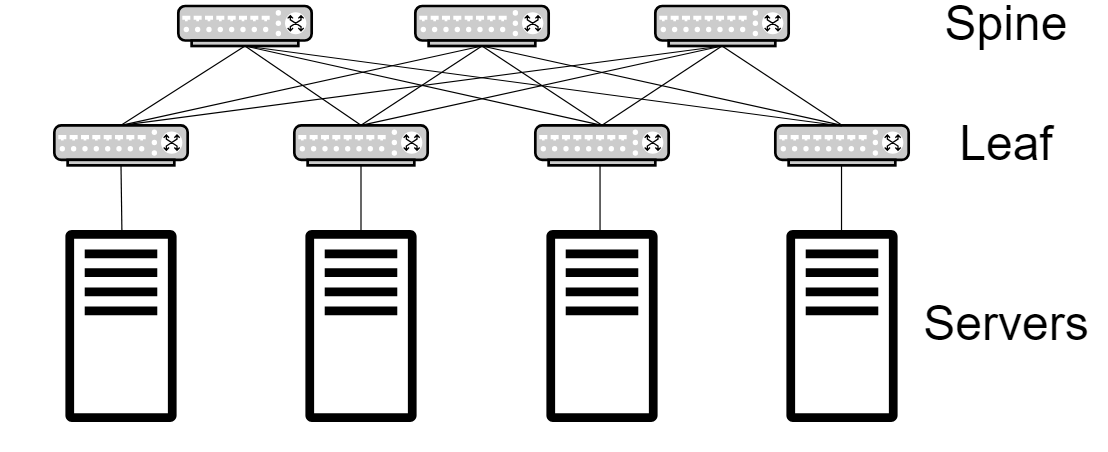
\includegraphics[width=0.6\linewidth]{images/ls.png}
    \caption{Leaf-spine architecture}
\end{figure}
Spine-leaf topologies draw inspiration from the realm of telephony, introducing a non-folded Clos structure.
This architecture features fully interconnected stages, ensuring that each matrix within one stage is linked, at least once, to every matrix in the subsequent stage, and vice versa.

\paragraph*{Clos networks}
Let's denote $k$ as the number of middle stage switches and $n$ as the number of inputs and outputs of switches in the side stages.
If $k\geq n$, there always exists a method to reorganize communications, allowing for the creation of a path between any pair of inactive input/output channels.
Moreover, if $k\geq 2n-1$, a path between any pair of idle input/output channels is guaranteed to be available.
It's important to note that $t$ serves as a flexible design parameter. 
Consequently, the total number of input/output channels,$ N=t\cdot n$, can be adjusted freely by increasing the size of middle-stage switches.
However, it's crucial to remember that a Data Center Network (DCN) operates as a packet-switched network.
\begin{figure}[H]
    \centering
    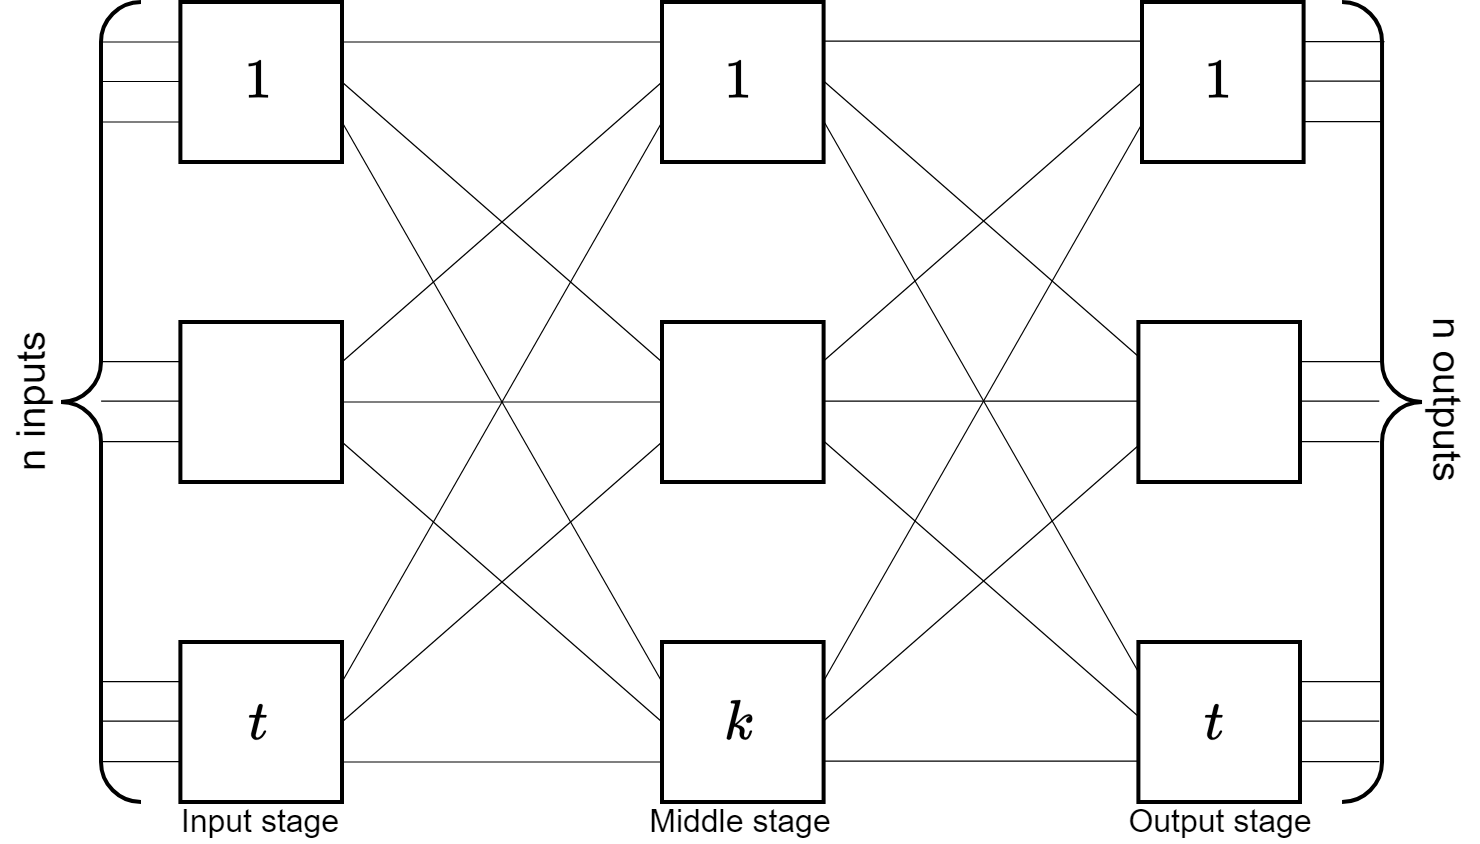
\includegraphics[width=0.6\linewidth]{images/stage.png}
    \caption{Clos network}
\end{figure}
In the Clos topology, where $n=m=k$, each switching module functions uni-directionally with $k$ input and $k$ output ports per module. 
The central stage comprises $k$ matrices, while the side stages consist of $t$ matrices. 
Path traversal encompasses three modules.

In the Leaf and Spine topology, every switching module operates bidirectionally: 
\begin{itemize}
    \item Leaf Configuration: comprises $t$ switching modules, each featuring $2k$ bidirectional ports per module.
    \item Spine Configuration: consists of $k$ switching modules, with each module having $t$ bidirectional ports.
\end{itemize}
In both configurations, paths traverse either one or three modules.

\paragraph*{Advantages}
The Clos design in Data Center Networks (DCNs) offers several advantages:
\begin{itemize}
    \item Utilization of homogeneous equipment throughout the network, simplifying management and maintenance.
    \item Routing serves as the Fundamental Interconnect Model, eliminating the need for Learning and Forwarding or Spanning Tree Protocol (STP).
    \item Implementation of Equal Cost Multipath (ECMP) strategy with routing protocols like IS-IS, SPB, or TRILL, enhancing network efficiency and resilience.
    \item Consistent number of hops for any pair of nodes, ensuring predictable and reliable communication.
    \item Small blast radius, minimizing the impact of network issues and failures.
\end{itemize}

\paragraph*{Upscaling}
We begin with a two-tier network structure and introduce an additional row of switches. 
Alternatively, we can consider transforming each spine-leaf group into a pod and incorporate a super spine tier. 
This architecture represents a highly scalable and cost-effective Data Center Network (DCN) design, focusing on optimizing bisection bandwidth. 
It can be constructed using standard Gigabit Ethernet switches with identical port counts. 
This approach is adopted by major tech giants like Microsoft and Amazon.
\begin{figure}[H]
    \centering
    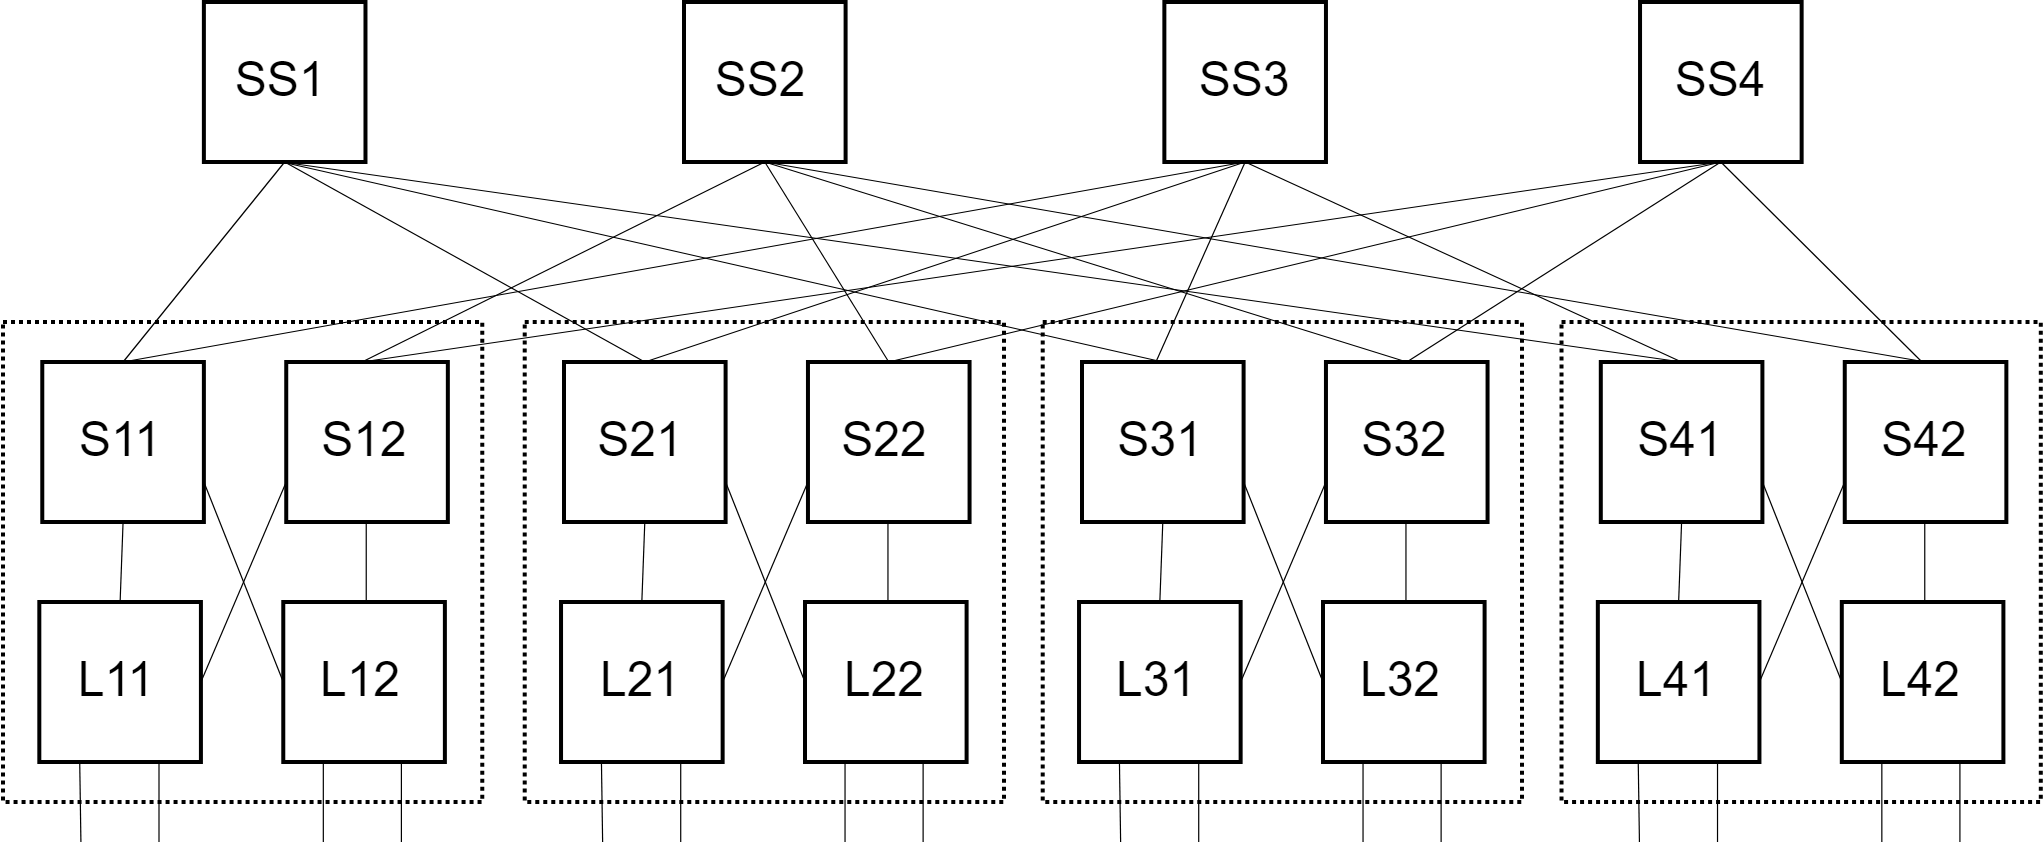
\includegraphics[width=0.6\linewidth]{images/pod.png}
    \caption{Pod-based three-tier Clos}
\end{figure}
A Point Of Delivery (POD) refers to a module or cluster comprising network, compute, storage, and application elements collaboratively functioning to provide a network service. 
The POD represents a standardized and replicable pattern, with its constituent components enhancing the modularity, scalability, and manageability of data infrastructure.

\paragraph*{Generalization of the architecture}
A leaf with $2k^2$ bidirectional ports is configured with $k$ ports connecting to servers and $k$ ports linking to the data center network. 
It's important to note that this setup cannot directly interconnect $2k^2$ servers as it would lead to network blocking. 
This configuration is constructed using $2k$ switches with $2k$ ports each.

The Point Of Delivery (PoD) is replicated $P$ times, each consisting of $k$ servers and $2P$ switches with $2k$ ports, and $k$ switches with $P$ ports. 
In a Fat-tree design, choosing $P=2k$, we have $2k^3$ servers, $5k^2$ switches with $2k$ ports each, and $2k$ PoDs at the edge layer, each containing $2k^2$ servers.

At the edge layer, each edge switch is directly connected to $k$ servers in a pod and $k$ aggregation switches. 
A fat-tree network with $2k$-port commodity switches can accommodate a total of $2k^3$ servers. 
Additionally, there are $2k^2$ core switches with $2k$-port each, with each one connected to $2k$ pods. 
Each aggregation switch is connected to $k$ core switches, highlighting partial connectivity at the switch level.

\paragraph*{VL2 network}

The VL2 Network is an economical hierarchical fat-tree-based Data Center Network (DCN) architecture designed to provide high bisection bandwidth. 
It employs three types of switches: intermediate, aggregation, and top-of-rack (ToR) switches.

The network comprises $\frac{D_A}{2}$ intermediate switches, $D_I$ aggregation switches, and $\frac{1}{2}D_A D_I$ ToR switches. 
The total number of servers in a VL2 network is calculated as $20\frac{D_A D_I}{4}$. 
A key feature of the VL2 Network is its use of a load-balancing technique called valiant load balancing (VLB).

\subsection{Switches}
Commodity switches are known for their affordability and simplicity, as well as their rapid evolution. 
While they offer intermittent capacity, they are suitable for scenarios where only a single operator is involved. 
On the other hand, WAN switches are more complex and expensive, with slower evolution. 
They provide the highest level of availability and allow intermittent capacity, with numerous protocols available to support interoperability among multivendor WANs.

\subsection{Server-centric and hybrid architectures}
A server-centric architecture, proposed for constructing containerized data centers, aims to lower implementation and maintenance expenses by solely utilizing servers to establish the DCN.\@ 
It employs a 3D-Torus topology to directly interconnect the servers, leveraging network locality to enhance communication efficiency. 
However, drawbacks include the necessity for servers with multiple Network Interface Cards (NICs) to assemble a 3D Torus network, as well as the presence of lengthy paths and heightened routing complexity.